%\newpage
\subsection{HELPFILE}
%           --------
\label{sec:helpfile}
%%%%%%%%%%%%%%%%%%%%%%%%%%%%%%%%%%%%%%%%%%%%%%%%%%%%%%%%%%%%%%%%%%%%%%%%%%%%%
%%%                             Description                               %%%
%%%%%%%%%%%%%%%%%%%%%%%%%%%%%%%%%%%%%%%%%%%%%%%%%%%%%%%%%%%%%%%%%%%%%%%%%%%%%
\subsubsection{Description}
You can give any number of help text files to be made available to the user
 via the help menu button. \index{help}
\INTENS{} provides two methods for displaying these files:
\begin{itemize}
\item display a simply structured text file in a special help window
       (see chapter \nameref{sec:hfintens}).
\item display a HTML\footnote{Hypertext Markup Language} file in the web browser
      which will be started if not already running
      (see chapter \nameref{sec:hfbrowser}).
\end{itemize}

\label{sec:hfdescription}
\input{diagrams/helpfile_description}
\index{HELPFILE@\HELPFILE}

\index{OPEN\_FILE@\OPENFILE!helpfile}
\index{OPEN\_URL@\OPENURL!helpfile}
\begin{tabularx}{\textwidth}{l|X}
help\_description        & description \\
\hline
\verb+filename_string+   & string: Name of a helpfile
                           (see chapter \nameref{sec:hfintens}). \\
\verb+document_string+   & string: Name (address) of a document \\
\OPENFILE                & connect to the web browser and open the specified file
                           (see chapter \nameref{sec:hfbrowser}). \\
\OPENURL                 & connect to the web browser and open the specified document
                           by loading it from a WWW server (see chapter \nameref{sec:hfbrowser}). \\
\end{tabularx}

%%%%%%%%%%%%%%%%%%%%%%%%%%%%%%%%%%%%%%%%%%%%%%%%%%%%%%%%%%%%%%%%%%%%%%%%%%%%%
%%%                            INTENS Help-Files                          %%%
%%%%%%%%%%%%%%%%%%%%%%%%%%%%%%%%%%%%%%%%%%%%%%%%%%%%%%%%%%%%%%%%%%%%%%%%%%%%%
%%%\newpage
\subsubsection{\INTENS{} Helpfiles}
\label{sec:hfintens}
These text files contain unformatted ASCII texts \index{help!ASCII text}
combined with some control
information:
\begin{itemize}
\item The first line must begin with \verb+#+. The characters immediately
       following until the end of that line
       will be used as title string.
\item Lines beginning with a period define a new chapter. The following
      text on the same line will be used as chapter head.
\item Lines beginning with a colon just after a chapter line define help keys.
      These help keys can be connected with forms (see chapter
       \nameref{key:helpkey} on page \pageref{key:helpkey}).
\end{itemize}

\newpage


\begin{boxedminipage}[t]{\linewidth}
\begin{verbatim}
#INTENS
.Overview
Each INTENS application is created through a simple script which
contains the configuration commands for the applications data
exchange interfaces between RDBMS, calculation programs, user
interface, printer and file system.
.Parser
:PARSE
The Parser interpretes at program startup the configuration data
and sends the appropriate messages to all involved objects to
create the application with all configured interfaces.
.Datapool
  ...
\end{verbatim}
\end{boxedminipage}


\vspace{0.5cm}

\index{  @Signs / Characters!\# (hash)!helpfile title}
\index{  @Signs / Characters!. (dot)!helpfile chapter}
\index{  @Signs / Characters!: (colon)!helpfile key}
\begin{tabularx}{\textwidth}{l|X}
help\_file & description \\
\hline
\verb+#+   & begin of file and title string \\
\verb+.+   & begin of chapter and chapter label \\
\verb+:+   & help key (\nameref{key:helpkey} page \pageref{key:helpkey}) \\
\end{tabularx}

\begin{figure}\label{fig:helpfile}
   \begin{center}
      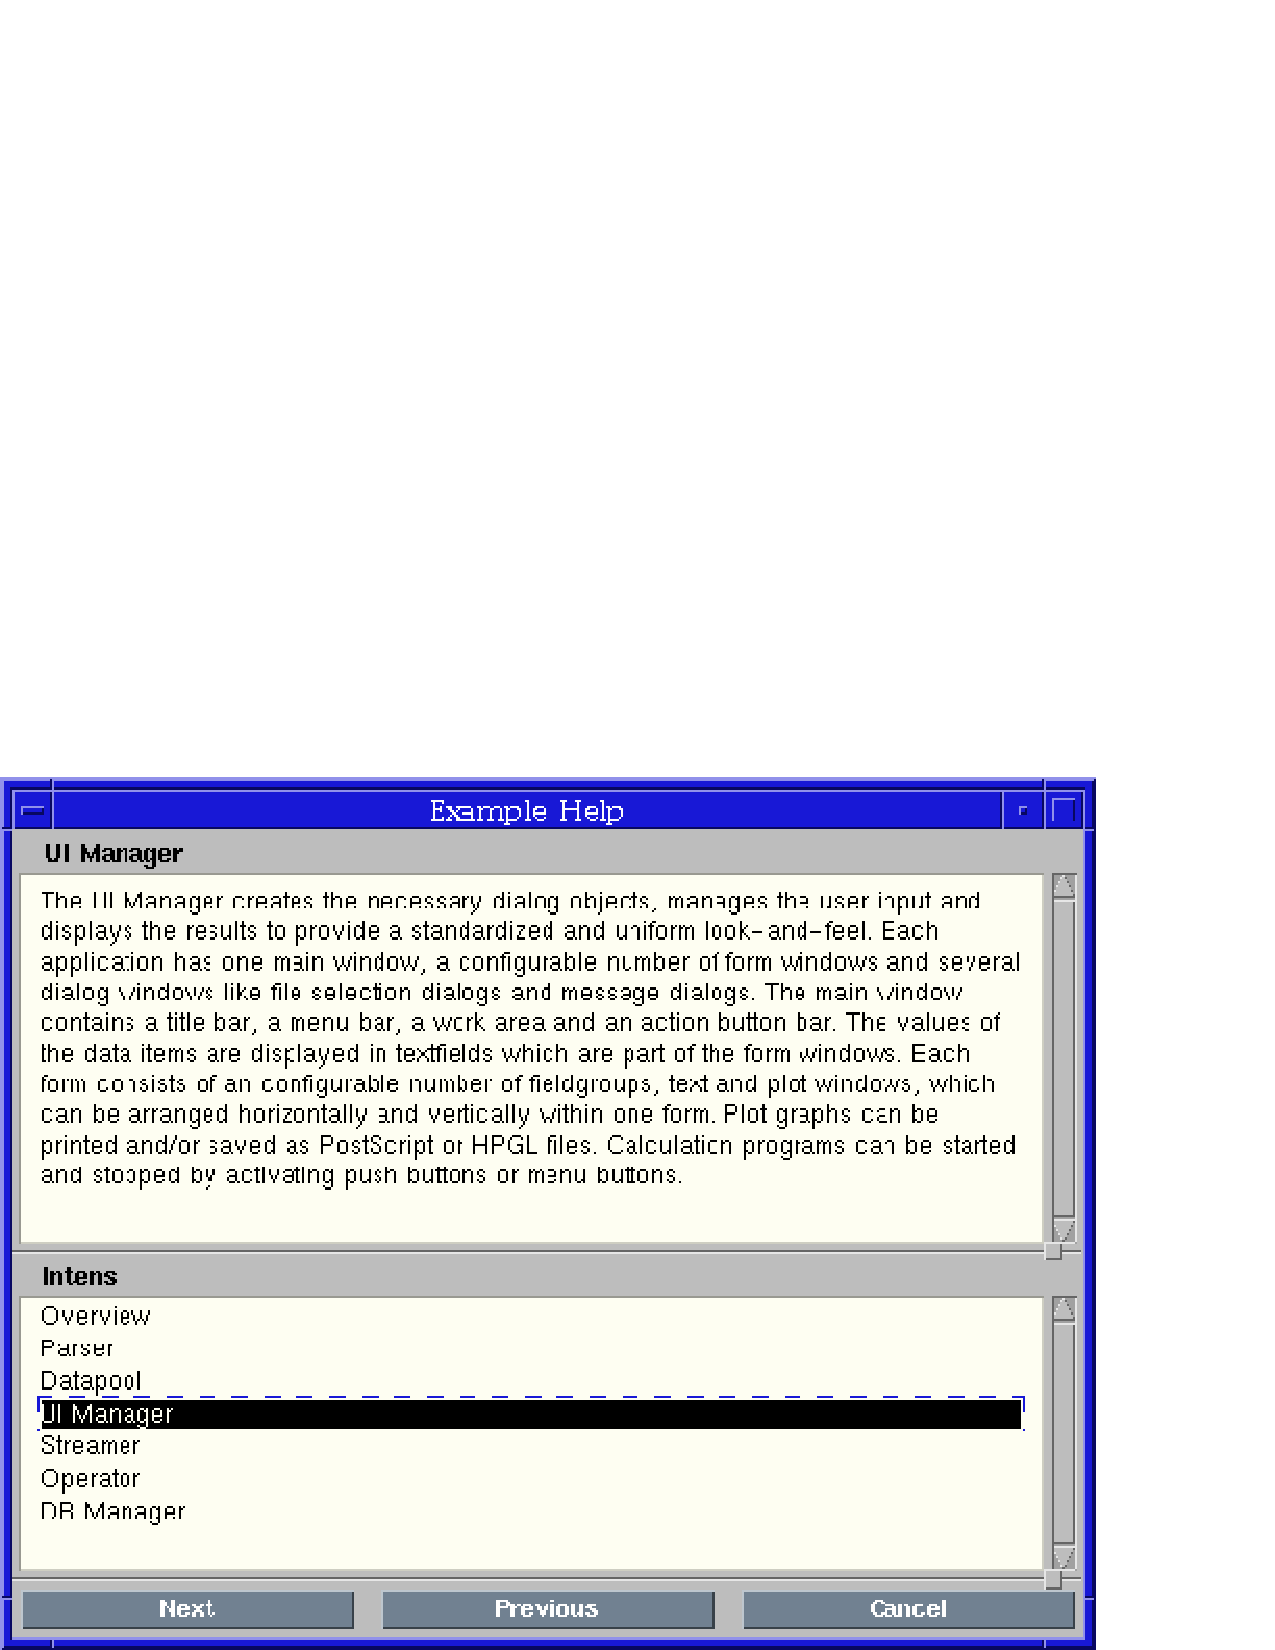
\includegraphics[width=13cm]{grab_helpfile}
   \end{center}
\caption{Example of a Help Window}
\end{figure}

%%%%%%%%%%%%%%%%%%%%%%%%%%%%%%%%%%%%%%%%%%%%%%%%%%%%%%%%%%%%%%%%%%%%%%%%%%%%%
%%%                               HTML                                   %%%
%%%%%%%%%%%%%%%%%%%%%%%%%%%%%%%%%%%%%%%%%%%%%%%%%%%%%%%%%%%%%%%%%%%%%%%%%%%%%
\newpage
\subsubsection{HTML files}
\label{sec:hfbrowser}
For displaying HTML files with the web browser \index{help!Web Browser}
either use \OPENFILE{} or \OPENURL. The specified file
must have a browser readable format such as HTML. \index{help!HTML}
The only thing \INTENS{} does is connecting to the web browser and invoking its open
command (with the \verb+-remote+ command).

\input{diagrams/helpfile_options}
\input{diagrams/helpfile_key}
\index{HELPFILE@\HELPFILE!options}
\index{HIDDEN@\HIDDEN!helpfile option}
\index{HELPKEY@\HELPKEY!helpfile option}

\begin{tabularx}{\textwidth}{l|X}
help\_options        & description \\ \hline
\verb+title_string+  & string: Defines the label in the help menu.
                       The filename is used if there is no title defined.\\
\HIDDEN              & No menu entry will be created for this helpfile.\\
\HELPKEY             & specifies the helpkeys (anchors) that are defined in the HTML file
                       (see chapter \nameref{key:helpkey} on page \pageref{key:helpkey}). \\
\end{tabularx}
\vspace{0.5cm}

If you want to reference specified anchors in your document, then you have
to list them as \HELPKEY s.
The following example shows an anchor named "goHere" in a HTML document:


\begin{boxedminipage}[t]{\linewidth}
\begin{verbatim}
...
<A NAME="goHere"<\A>
...
\end{verbatim}
\end{boxedminipage}


%%%%%%%%%%%%%%%%%%%%%%%%%%%%%%%%%%%%%%%%%%%%%%%%%%%%%%%%%%%%%%%%%%%%%%%%%%%%%
%%%                              Examples                                 %%%
%%%%%%%%%%%%%%%%%%%%%%%%%%%%%%%%%%%%%%%%%%%%%%%%%%%%%%%%%%%%%%%%%%%%%%%%%%%%%
%%\subsubsection{Examples}
\label{sec:helpfileexamples}


\begin{boxedminipage}[t]{\linewidth}
\begin{alltt}
\HELPFILE
  "helpfile.hlp",
  "helpfile\_2.hlp",
  OPEN\_FILE "helpfile.html"  HELPKEY("goHere"),
  OPEN\_URL  "www.semafor.ch"
;
\end{alltt}
\end{boxedminipage}
